\chapter{Physics: Statistical Physics}\label{ch:statphys}

One regime of interest for lattice QCD calculations is the application
of lattice formalism to hot, dense nuclear systems; this is the realm
of thermodynamics\index{thermodynamics} and statistical physics. In this chapter I try to
offer some reminders of statistical physics, especially those that
are directly relevant to modern lattice investigations of the QCD
phase diagram. Some references I drew from include
Ref.~\cite{tahir-kheli_general_2012} and \cite{kardar_statistical_2007}.

\section{A brief history of early thermodynamics}

As it turns out, much of thermodynamics was discovered in order to develop
and increase the efficiency of engines. This presentation is based
on Ref.~\cite{wiki:thermo}. The first engine progenitor that I'm
aware of would be the vacuum pump, which was built and designed by Otto von 
Guericke in 1650. Shortly thereafter, Boyle and Hooke developed an air pump.
Playing around with this air pump helped reveal {\it Boyle's law}\index{Boyle's
law}
\begin{equation}
  P\propto\frac{1}{V},
\end{equation}
a relationship between the pressure $P$ and volume $V$ of a gas.

In 1697, Denis Papin developed a steam digester, a closed vessel which trapped steam 
until a high pressure was generated, with a valve to release pressure to keep it
from exploding.  He noticed the value would rhythmically move up and down and was 
inspired to create a piston and cylinder engine; however, he did not pursue this design. 
In 1712, Thomas Newcomen built the first engine based on Papin's concept.
This\index{engine!Newcomen} {\it Newcomen engine} was quite inefficient; by
1781, major improvements were made by James Watt, including making the condenser a separate
entity to avoid energy loss repeatedly cooling and re-heating the cylinder and
implementing rotary motion, allowing the\index{engine!Watt} {\it Watt engine} to 
be more broadly applicable.
Such early engines are examples of {\it external combustion engines}, which
burn\index{engine!external combustion}
fuel, using the heat to increase the temperature of some liquid whose
pressurized vapor is used to move something.

The development of thermodynamics as a modern science arguably begins with
with Sadi Carnot, who in 1824 published {\it Reflections on the Motive Power of
Fire}, a text on heat, power, energy and engine efficiency. 
His book outlined energetic relations between the\index{Carnot!engine}
Carnot engine, the\index{Carnot!cycle} Carnot cycle, and motive power. 
In 1850, Clausius published a paper titled ``On the Moving Force of Heat", which 
first stated the basic principles of the second law of thermodynamics. 
He introduced the concept of entropy\index{entropy} in 1865.

In parallel to the development of thermodynamics as a discipline was the
constant improvement of commercial engine efficiency. Of particular note for
modern transportation is the constant improvement of the {\it internal
combustion engine}\index{engine!internal combustion}, where the products of fuel
combustion themselves directly provide the pressure used to produce mechanical
motion. These improvements were due to many scientists and engineers and
happened over the course of many years~\cite{wiki:internalCE}.
A few notable engineers, which include some household names, are listed in
chronological order of their contributions:
In 1872, George Brayton invented the first commercial liquid-fueled 
internal combustion engine. In 1876, Nicolaus Otto, in cooperation with Gottlieb 
Daimler and Wilhelm Maybach, patented the four-stroke cycle engine with a 
compressed charge. Karl Benz, four years later in 1879, patented a 
dependable two-stroke gas engine. Lastly, in 1892 Rudolf Diesel\footnote{Diesel
engines tend to be more efficient for transportation 
than gas engines, in the sense that they tend
to deliver more distance per unit fuel. One of the reasons for this is that the
combustion is triggered by high pressure instead of a spark, which requires more
compression. When the gas then expands, it therefore pushes the piston a larger
distance. Diesel died under mysterious circumstances--one likely possibility is that he
was assassinated.} invented the 
first compressed charge, compression ignition engine.


\section{The laws of thermodynamics}

In thermodynamics, one usually divides the universe into a system 
(or collection of systems) under
consideration and its (their) surroundings.
The {\it zeroth law of thermodynamics} is just the statement that
equilibrium is transitive.\index{thermodynamics!zeroth law}
\begin{theorem}{Zeroth law of thermodynamics}{}
  If two systems $A$ and $B$ are in equilibrium with a system $C$, then
$A$ and $B$ are also in equilibrium.
\end{theorem}
Let $U$ be the energy of any system,
$Q$ the heat added to it, and
$W$ the work done on it. The {\it first law of thermodynamics}
is the statement of energy conservation.\index{thermodynamics!first law}
\begin{theorem}{First law of thermodynamics}{}
  $$\dd U=Q+W$$
\end{theorem}
%In other words, heat and work are the only ways to change a system's energy.

These two laws are relatively straightforward to understand. But to understand
the second law, one needs the concept of entropy. First we will proceed
using discoveries by Carnot and Clausius, which I think is valuable
because it helps one understand why $Q=T\dd S$. Then we will take a look at an
information-oriented understanding of entropy. Both of these follow the
presentations in Ref.~\cite{kardar_statistical_2007} closely.



\begin{figure}
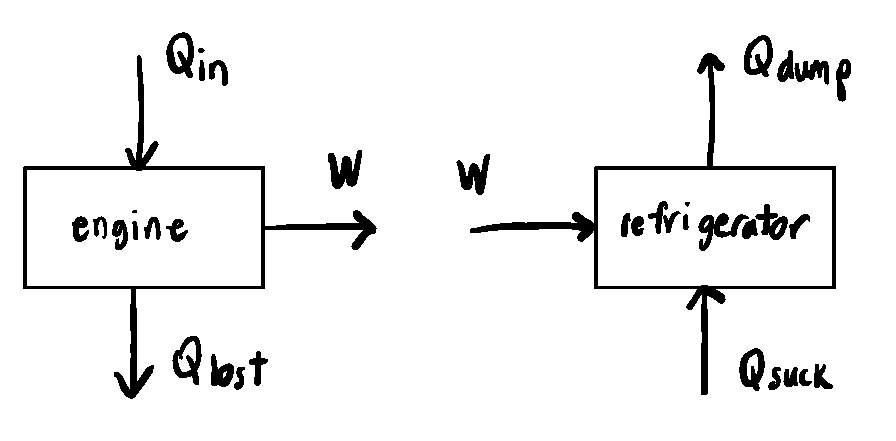
\includegraphics[width=\linewidth]{figs/engineFrige.pdf}
\caption{Schematic diagrams for an ideal engine (left) and refrigerator (right).}
\label{fig:engineFrige}
\end{figure}



\subsection{Entropy from engines}

A {\it heat engine}\index{engine!heat} is any idealized system that takes in
heat $\Qin$ from a source, converts some of that into work $W$, and loses some heat to its
surroundings $\Qlost$. A reasonable measure of its efficiency\footnote{It is not
clear to me at this stage that this is the ``best" definition of efficiency or a
unique one. In particular, one could raise this ratio of heat to an arbitrary
(positive) power. In a sense, using 1 as the power is the simplest possible definition. 
Additionally, when we derive
the Carnot engine efficiency, we will see that it related to the ratio
of two temperatures raised to some power. There also we have the freedom to
pick a power, and again the simplest decision is 1. Picking the same power for
the heat and the temperature ratios is important so that the entropy derived from
engines matches the microcanonical (or information) entropy, which we will derive
later.} is
\begin{equation}\label{eq:engineEff}
  \text{efficiency}=\frac{W}{\Qin}=\frac{\Qin-\Qlost}{\Qin}\leq1,
\end{equation}
where the inequality is due to the first law of
thermodynamics\footnote{Incidentally, this rules out any (perpetual motion)
machine that can produce more energy than you put in.}.
A {\it refrigerator}\index{refrigerator} is any idealized system that does the
opposite; i.e. it takes in some work $W$ to suck some heat $\Qsuck$ out of
some source, and dumps that heat $\Qdump$ into its environment.
Similarly, a reasonable measure of the refrigerator's efficiency is
\begin{equation}\label{eq:refrigeratorEff}
  \text{efficiency}=\frac{\Qsuck}{W}=\frac{\Qsuck}{\Qdump-\Qsuck},
\end{equation}
Schematics of an ideal engine and refrigerator are given in
\figref{fig:engineFrige}.
With this terminology, we give two equivalent statements of the second law,
which as far as I can tell, are just things that were empirically observed
when developing engines:\index{thermodynamics!second law}
\begin{enumerate}
  \item (Kelvin) There is no process whose sole result is the conversion of heat
        into work. In other words the inequality in \equatref{eq:engineEff}
        should be strict.
  \item (Clausius) There is no process whose sole result is the transfer of
        heat from a colder system to a warmer one. In other words, the
        efficiency \eqref{eq:refrigeratorEff} is finite.
\end{enumerate}
It is not too difficult to show using ideal engines and refrigerators
that these two formulations are equivalent~\cite{kardar_statistical_2007}.
Later, we will formulate these in terms of a new quantity, entropy. The
formulation in terms of entropy can be proven in the framework of statistical
physics.

In order to examine systems in detail, we need to be in equilibrium so that all
thermodynamic coordinates are well defined.
If nothing changes, a system remains in equilibrium; it stands to reason that
if a process happens sufficiently slowly, it is more or less still in
equilibrium. Such processes are called\index{quasistatic} {\it quasistatic}.
A process is {\it adiabatic}\index{adiabatic} if $Q=0$ throughout that process.

Next we introduce the idea of a\index{engine!Carnot} {\it Carnot engine},
which should theoretically be the most efficient engine possible. 
It turns out that the most important property of such an engine is that it 
is\index{reversible} {\it reversible}, i.e. that you can reverse all its inputs
and outputs with the result that it works like the forward engine running
backwards in time. In particular a Carnot engine is reversible,
runs\index{cycle} in a {\it cycle}, i.e. it returns to its original state
at the end of its process, and its heat exchanges occur at 
temperatures\footnote{A Carnot cycle generically consists of two adiabats
and two isotherms. Specifying the heat exchanges at these temperatures allows us
to pick two isotherms. One can theoretically find adiabats using, e.g. an ideal
gas, but in principle Carnot engines with other materials are possible.}
$T_H$ and $T_C$, i.e. it draws and dumps heat without changing the
temperatures of its surroundings.
Looking at \figref{fig:engineFrige}, we see that a Carnot
engine run backward in time is just a Carnot refrigerator, and vice versa.

\begin{figure}
\centering
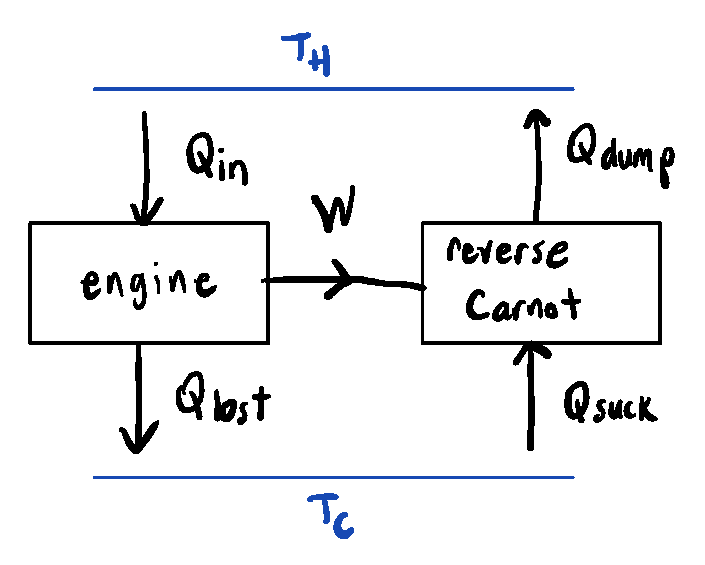
\includegraphics[width=0.7\linewidth]{figs/carnotThm.pdf}
\caption{An idealized machine used to prove Carnot's theorem.}
\label{fig:carnot}
\end{figure}

To see why this reversibility matters, consider \figref{fig:carnot}. In this
system, we use any engine to draw heat from a hot reservoir fixed at
$T_H$ that loses heat to a cold reservoir $T_C$ with $T_H>T_C$. We reverse a Carnot engine,
and use the output work from the left engine as input work to the reversed
Carnot engine. This combined system works as a process whose sole result 
transfers heat between the top and bottom reservoirs. By Clausius's statement 
of the second law of thermodynamics, it must be that $\Qin\geq\Qdump$ and
$\Qlost\geq\Qsuck$. It follows that
\begin{equation}
\text{efficiency}=\frac{W}{\Qin}\leq\frac{W}{\Qdump}=\text{Carnot engine
efficiency}.
\end{equation}

\index{Carnot's theorem}
\begin{theorem}{Carnot}{}
No engine is more efficient than a Carnot engine.
\end{theorem}

\begin{corollary}{Carnot}{carnot}
All Carnot engines have the same efficiency $\eta(T_H,T_C).$
\end{corollary}

\begin{figure}
\centering
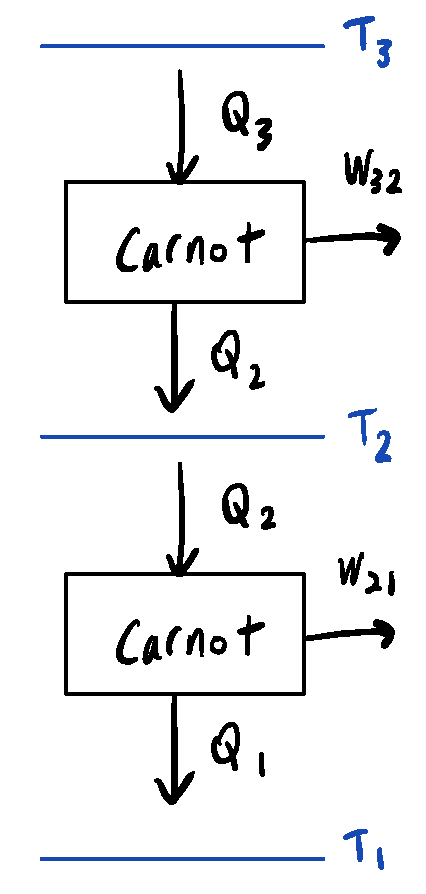
\includegraphics[width=0.6\linewidth]{figs/carnotSeries.pdf}
\caption{A series of Carnot engines.}
\label{fig:carnotSeries}
\end{figure}

Next, we are going to derive a relationship between heat flow and reservoir
temperature for the Carnot engine. Once we have this relationship, we will
creatively apply our knowledge of Carnot engines to say something about heat
flow and temperature generally. This will ultimately lead us to conclude that
entropy exists, and deliver a definition of it.

To derive the aforementioned relationship, consider a series of Carnot engines
as shown\footnote{The Carnot engines are identical and reversible, so it
must be that the heat exchanges on either side of $T_2$ are the same.}
in \figref{fig:carnotSeries} with $T_3>T_2>T_1$. The total effect of this
Carnot series is to take in heat $Q_3$, lose heat $Q_1$, and do work
$W_{31}=W_{32}+W_{21}.$ Using \corref{cor:carnot} 
we find that the heat exchanges must be related by
\begin{equation}\begin{aligned}
  Q_2 &= Q_3 - W_{32} &&= Q_3\left(1-\eta(T_3,T_2)\right) \\
  Q_1 &= Q_2 - W_{21} &&= Q_2\left(1-\eta(T_2,T_1)\right) 
                  = Q_3\left(1-\eta(T_3,T_2)\right)\left(1-\eta(T_2,T_1)\right) \\
  Q_1 &= Q_3 - W_{31} &&= Q_3\left(1-\eta(T_3,T_1)\right).
\end{aligned}\end{equation}
From the last two equations, it follows
\begin{equation}
\left(1-\eta(T_3,T_2)\right)\left(1-\eta(T_2,T_1)\right) =
1-\eta(T_3,T_1).
\end{equation}
Whatever the functional form of $1-\eta$ is, the middle temperature must be
cancelled through a multiplication. Hence $1-\eta$ must be a ratio of its input
temperatures, raised to some power. The simplest choice\footnote{Again, this
choice also will help our definition of entropy match that from the
microcanonical ensemble.} that guarantees $0\leq\eta<1$ is
\begin{equation}\label{eq:carnotEfficiency}
  \frac{Q_1}{Q_2}=1-\eta(T_2,T_1)\equiv\frac{T_1}{T_2}.
\end{equation}

It is nice to have this expression for the Carnot engine efficiency.
But again, from my perspective, it's more interesting to have this relation between
heat and temperature at the input and output heat vents for the engine.
Indeed, we can now potentially learn something about heat delivered
to an arbitrary system at some temperature, and we will leverage this trick to
prove a theorem due to Clausius.

\begin{figure}
\centering
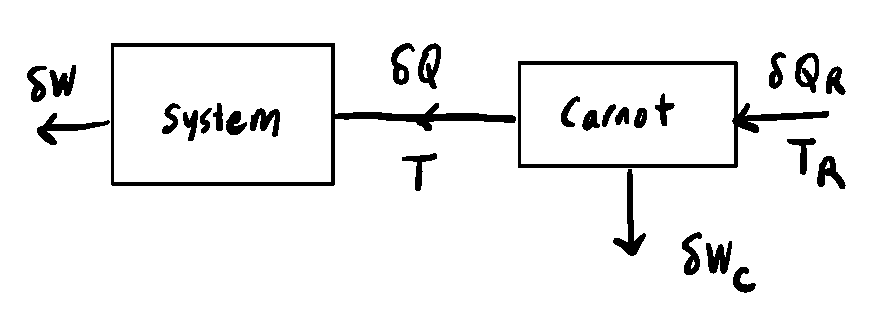
\includegraphics[width=\linewidth]{figs/clausius.pdf}
\caption{A convenient setup used to prove Clausius's theorem.}
\label{fig:clausius}
\end{figure}

\index{Clausius's theorem}
\begin{theorem}{Clausius}{}
For any cyclic transformation,
$$ \oint\frac{\delta Q}{T}\leq0. $$
where $\delta Q$ is a small amount of heat supplied at temperature $T$ to
a system during part of the cycle.
\begin{proof}
Consider the setup of \figref{fig:clausius}. The directions of heat and
work can be chosen as given WLOG. We begin with a system that
has a small amount of heat $\delta Q$ delivered to it at temperature $T$; by
energy conservation, some work $\delta W$ will leave the system.
To leverage \equatref{eq:carnotEfficiency}, we direct $\delta Q$ to the output port
of a Carnot engine, which generically takes in heat $\delta Q_R$ from a
reservoir at temperature $T_R$ and does some work $\delta W_E$.
From \equatref{eq:carnotEfficiency} we have
\begin{equation*}
\delta Q_R=T_R\frac{\delta Q}{T}.
\end{equation*}
After returning to their original states, the system and Carnot engine have the
combined effect of taking in heat $Q_R=\oint\delta Q_R$ and doing work $W$.
By energy conservation $Q_R=W$. By Kelvin's statement of the second law, it must
be that positive work is done on the system and positive heat leaves
the system; given our arrow conventions, we conclude $W=Q_R\leq0$. Hence
\begin{equation*}
T_R\oint\frac{\delta Q}{T}\leq0.
\end{equation*}
That $T_R$ is non-negative proves the theorem.
\end{proof}
\end{theorem}

We are finally in a position to define\index{entropy} entropy.
In particular, if we further specify that the cycle is reversible,
we will find that $\delta Q\to-\delta Q$ when we switch the direction of the
cycle. It follows that for a reversible cycle
\begin{equation}
 \oint\frac{\delta Q}{T}=0. 
\end{equation}
This tells us that the process is path-independent, which means we can define a
new function $S$ with
\begin{equation}
 S(B)-S(A)=\int_A^B\frac{\delta Q}{T}. 
\end{equation}
Hence we learn for reversible\footnote{I've seen examples of people defining
reversible\index{reversible} systems to be those that have $Q=T\dd S$.}, 
quasistatic\footnote{Lattice calculations are always done under the assumption
of equilibrium, which means it's quasistatic by definition.} changes
\begin{equation}
Q=T\dd S.
\end{equation}
It follows that reversible, adiabatic processes are\index{isentropic} isentropic.
We also get this statement of the first law:\index{thermodynamics!first law}
\begin{equation}
 \dd U = T\dd S+P\dd V.
\end{equation} 

Finally, consider a possibly irreversible path from $A$ to $B$ that is closed
with a reversible one from $B$ to $A$. From Clausius's theorem, we get
\begin{equation}
\int_A^B\frac{\delta Q}{T}+\int_B^A\delta Q_{\text{rev}}\leq0
\end{equation}
or
\begin{equation}
\int_A^B\frac{\delta Q}{T}\leq S(B)-S(A).
\end{equation}
It follows that $\delta S\geq\delta Q/T$ for any process. In particular consider
two systems that are originally isolated from each other and separately in
equilibrium, then allow them to exchange heat. Since there is no work, we must
have $\delta Q_{\text{total}}=0$ by the first law, and hence $\delta
S_{\text{total}}\geq0$. This is the more familiar statement of
the {\it second law of thermodynamics}.\index{thermodynamics!second law}
\begin{theorem}{Second law of thermodynamics}{}
If two or more adiabatically isolated systems are brought into thermal contact,
their combined entropy must always increase.
\end{theorem}

In the context of statistical physics, this statement will follow from
probabilistic considerations. There we will see that systems in equilibrium have
maximum entropy. What about statements of minimum entropy? This is covered by
the {\it third law of thermodynamics}, which is an observation.\index{thermodynamics!third law}
\begin{theorem}{Third law of thermodynamics}{}
$$
  \lim_{T\to0}S(T)=0
$$
\end{theorem}


\subsection{Entropy from information}

\section{Equations of state}\label{sec:EoS}


Probably the equation of state that you are most familiar with is the 
ideal gas law,\index{ideal gas law}
\begin{equation}
  PV=NkT.
\end{equation}
The volume $V$ and the number of particles $N$ both scale linearly with the
size of the system; we call such variables {\it extensive}\index{extensive}. 
Meanwhile the pressure $P$ and the temperature $T$ are {\it intensive}\index{intensive}, 
i.e. they do not scale with the system.

There is an equation of state for each intensive variable required for the
description of thermodynamic states. For example from the
first law of thermodynamics,\index{thermodynamics!first law}
\begin{equation}\label{eq:fslaw}
  \dd{U}=T\dd{S}-P\dd{V}+\sum_i\mu_i\dd{N}_i,
\end{equation}
we know that\footnote{It can be quite confusing to track which variables
are held fixed and allowed to vary doing these partial derivatives.
This matters because sometimes different choices of control parameters
are related to each other through a constraint.
You can get a hint for example by looking at equations like
\equatref{eq:fslaw}, which is a reminder we are thinking of
$U$ as a function of the set \{$S$, $V$, $\vec{N}$\}. In this context,
partial derivatives with respect to one of those variables must
guarantee the others in that set are fixed.}

\begin{equation}
  T=\pdv{U}{S}.
\end{equation}
This intensive variable $T$ depends on only the extensive variables; 
generally we could write
\begin{equation}
  T=T(U,S,V,N).
\end{equation}
This is what we call an {\it equation of state}\index{equation of state}
(EoS). The arguments are sometimes referred to as 
{\it control parameters}\index{control parameter}. Knowing every equation 
of state is enough to reconstruct the fundamental equation, and therefore 
enough to determine the physics of the system.

\section{Legendre transforms}\index{Legendre transformation}

Equation~\eqref{eq:fslaw} tells us that we can think of the internal energy
$U$ of a system in equilibrium at $(T,P,\mu)$ as a function of $S$, $V$, and
$N$. However one of the control parameters, such as $S$, may be
difficult or impossible to measure, and therefore we would rather
think in terms of the more accessible quantity $T$, which 
is the derivative of $U$ with respect to $S$; 
Hence we want 
\begin{enumerate}
\item to look at $U$ in terms of a derivative with respect to $S$ rather 
      than $S$ itself; moreover 
\item we don't want to lose any information we had before, i.e. we want this
      process to be invertible. 
\end{enumerate}
These are the purposes of a Legendre transformation. The second point 
may seem too obvious to state, but it's worth emphasizing here because 
what makes thermodynamic potentials such as $U$ special is that you're 
supposed to be able to determine state variables like $T$ from them. 
Since no information is lost, Legendre transforms guarantee that 
thermodynamic potentials get transformed to other thermodynamic potentials.
\index{thermodynamic!potential}\index{potential!thermodynamic}

Before we define a Legendre transformation, let's look at an example
due to Markus Deserno~\cite{deserno} where a naive transformation can go
wrong and information can be lost. 
\begin{example*}{}
We consider a function $y(x)$ and define a new variable
\begin{equation}\label{eq:xlegendre}
  p\equiv y'(x).
\end{equation}
In order to accomplish goal (1) above, one might naively solve
\equatref{eq:xlegendre} for $x$, obtaining the function $x(p)$
and then plug this back into $y(x)$ to obtain
\begin{equation}
  Y(p)=y\left(y'^{-1}(p)\right).
\end{equation}
To see that this procedure destroys information, consider the example
\begin{equation}\label{eq:badlegendre}
  y(x)=\frac{1}{2}(x-x_0)^2.
\end{equation}
The derivative is $p=y'(x)=x-x_0$, and hence $x=p+x_0$. Plugging this
into \equatref{eq:badlegendre} we get the function
\begin{equation}
  Y(p)=y(x(p))=\frac{1}{2}\left(x(p)-x_0\right)^2=\frac{1}{2}p^2.
\end{equation}
Evidently all functions of the form~\eqref{eq:badlegendre} get transformed
to the same function regardless of the value of $x_0$; therefore there is
no way starting from $Y(p)$ to figure out what $x_0$ was. Hence
information was destroyed.
\end{example*}

Now on to the definition. Recall that a function $f$ is {\it convex}
\index{function!convex} in a region if the graph of the function lies 
below the line segment connecting any two points in that region. It is 
{\it concave}\index{function!concave} if $-f$ is convex. Consider
a function $y:\R\to\R$. Then the 
{\it Legendre transform} is defined by
\begin{equation}
Y(p)=\begin{cases}
  \min_x [y(x)-xp] & \text{if $y$ is convex}\\
  \max_x [y(x)-xp] & \text{if $y$ is concave.}
\end{cases}
\end{equation}
This definition makes sense in view of goal (1) at the beginning of this
section, assuming $y$ is differentiable. To see this, note that the maximum
or the minimum corresponds to a critical point, and so
\begin{equation}\label{eq:legendremin}
  0=\frac{d}{dx}\left[y(x)-xp\right]=y'(x)-p.
\end{equation}

We now state two useful facts about Legendre transforms. These can
be relatively straightforwardly proven. We emphasize that Legendre
transformations are only defined for concave or convex functions, and
that the concavity or convexity is important to prove the second point,
because it guarantees that the derivative is monotonic.
\begin{proposition}{}{}
  \begin{enumerate}
    \item The Legendre transformation of a convex function is concave
          and vice versa.
    \item The Legendre transformation is its own inverse.
  \end{enumerate}
\end{proposition}

Now that we have some intuition for why one might want to do a
Legendre transform, we are going to see how some other useful
thermodynamic potentials arise from carrying them out.

\subsection{Helmholtz free energy}
\index{free energy!Helmholtz}
Let us now return to our issue of dropping $S$ in favor
of $T$. According to the above section if we
Legendre transform $U(S)$ out of the variable $S$, then the minimization
will guarantee that the new independent variable is $T$. Calling
this new function $F$, we obtain
\begin{equation}\label{eq:helmholtz}
  F(V,T,N)=U-TS.
\end{equation}
This new function is guaranteed to be a thermodynamic potential, and
we give it a special name: the {\it Helmholtz free energy}.
From \equatref{eq:helmholtz} and the first law, we get
\begin{equation}\label{eq:helmholtz1st}
  \dd F = -P\dd V -S\dd T +\sum_i\mu_i\dd{N}_i.
\end{equation}

We can derive some useful thermodynamic relations from these. For
instance
\begin{equation}\label{eq:dfdt}
  -T^2\pdv{(F/T)}{T}=U=\pdv{(\beta F)}{\beta},
\end{equation}
where $\beta=1/T$ in natural units.


\subsection{Enthalpy}\index{enthalpy}

The {\it enthalpy} is given by the Legendre transformation
\begin{equation}\label{eq:enthalpy}
 H(S,P,N)=U+PV.
\end{equation}
From \equatref{eq:enthalpy} and the first law we obtain
\begin{equation}\label{eq:enthalpy}
 \dd H = T\dd S +V\dd P +\sum_i\mu_i\dd N_i.
\end{equation}


\section{Ideal quantum gas}

\subsection{Canonical formulation}

\index{gas!bose}\index{gas!fermi}
\begin{equation}
\eta=
  \begin{cases}
     +1 & \text{bosonic gas} \\
     -1 & \text{fermionic gas}.
  \end{cases}
\end{equation}

\subsection{Grand canonical formulation}

% keep discussion general to mu_i N_i
\index{fugacity}
\begin{equation}\label{eq:fugacity}
  z=e^{-N\mu/T}
\end{equation}

The {\it grand potential} is\index{grand potential}
\begin{equation}\label{eq:grand}
  \Phi\left(V,T,\vec{\mu}\right)=U-TS-\sum_i\mu_i N_i=-T\log\grandZ
\end{equation}
from which one gets
\begin{equation}\label{eq:1stlawgrand}
  \dd\Phi=-P\dd V-S\dd T-\sum_i N_i\dd\mu_i.
\end{equation}
Since $\log\grandZ$ is extensive, it must be that
\begin{equation}
-T\log\grandZ=kV
\end{equation}
for some intensive $k$. Hence\footnote{Sometimes it is convenient to work
with $\muh\equiv\mu/T$ and $T$ instead of $\mu$ and $T$. This equation
holds for both sets of control variables since both $\mu$ and $T$ are
held fixed.} from \equatref{eq:1stlawgrand}
\begin{equation}
P=-\pdv{\Phi}{V}=-k,
\end{equation}
which means we can identify
\begin{equation}\label{eq:pgrand}
P=\frac{T}{V}\log\grandZ.
\end{equation}

Reorganizing \equatref{eq:grand} using \equatref{eq:pgrand}
yields the {\it Gibbs-Duhem relation}
\index{Gibbs-Duhem relation}
\begin{equation}
  s=\frac{\epsilon}{T}+\frac{P}{T}-\sum_i\frac{\mu_i}{T}n_i,
\end{equation}
where $s\equiv S/V$ is the entropy density, and $\epsilon$ and $n_i$
are the energy and number densities.
Taking a derivative of \equatref{eq:pgrand} w.r.t. $\mu_i$ and
using \equatref{eq:1stlawgrand} yields
another often useful relation,
\begin{equation}
  \frac{N_i}{V}=\pdv{P}{\mu_i}.
\end{equation}

\section{Relativistic quantum gases}

Relativistic quantum gases are especially interesting for us
to consider because of their
application to low temperatures of the QCD phase diagram. There, the medium
behaves approximately like a relativistic gas of hadronic bound states.
This allows for a cross check against lattice QCD at low temperatures
and at finite densities. Following some lecture notes by F. Karsch,
we are going to derive the
pressure. From this we can derive other thermodynamic quantities
using standard thermodynamic relations.

We use units $\hbar=c=k_B=1$ and consider a gas of a single species
with spin $s$ and rest mass $m$. Working in the rest frame of the gas,
we have
\begin{equation}\label{eq:dispersion}
  E=\sqrt{p^2+m^2}.  
\end{equation}
From the grand canonical formulation,
doing the momentum integral in spherical coordinates, the pressure is
\begin{equation}
  \frac{P}{T}=-\frac{4\pi\eta g}{(2\pi)^3}\int_0^\infty 
      \dd{p}p^2\log\left(1-\eta z e^{-E/T}\right),
\end{equation}
where $g=2s+1$ is the {\it degeneracy factor}. \index{degeneracy factor}
Solving the dispersion relation
for $p$ and substituting it into the pressure gives
\begin{equation}
  \frac{P}{T}=-\frac{4\pi\eta g}{(2\pi)^3}\int_m^\infty 
      \dd{E}E\left(E^2-m^2\right)^{1/2}\log\left(1-\eta z e^{-E/T}\right).
\end{equation}
Expanding the logarithm yields
\begin{equation}\label{eq:pressE}
  \frac{P}{T}=\frac{4\pi g}{(2\pi)^3}\sum_{k=1}^\infty\eta^{k+1}\frac{z^k}{k}\int_m^\infty 
      \dd{E}E\left(E^2-m^2\right)^{1/2}e^{-kE/T},
\end{equation}
which is of course only valid for $\eta z\exp(-E/T)<1$.

Let us now evaluate the integral in \equatref{eq:pressE}. We introduce
$x\equiv E/m$. Performing this variable change and integrating by parts gives
\begin{equation}\label{eq:pressint}
  \int_m^\infty\dd{E}E\left(E^2-m^2\right)^{1/2}e^{-kE/T}
  =\frac{km^4}{3T}\int_1^\infty\dd x\left(x^2-1\right)^{3/2}e^{-mkx/T}.
\end{equation}
This integral can now be expressed in terms of the
{\it modified Bessel functions}\index{Bessel function!modified}
\begin{equation}
  K_\nu(a)=\frac{\pi^{1/2}(a/2)^\nu}{\Gamma(\nu+1/2)}
             \int_1^\infty\dd x(x^2-1)^{\nu-1/2}e^{-ax}.
\end{equation}
In particular we see upon comparison with \equatref{eq:pressint}
that our integral contains $K_2(mk/T)$. Combining everything,
using $\Gamma(5/2)=3\pi^{1/2}/4$, we obtain
\begin{equation}\label{eq:pressrelQM}
  \frac{P}{T}=\frac{m^2gT}{2\pi^2}\sum_{k=1}^\infty\frac{\eta^{k+1}z^k}{k^2}
                         K_2\left(\frac{mk}{T}\right),
\end{equation}
which is a form that is well suited for computer calculations\footnote{What
one does is keep some number of terms of the above sum, usually depending
on the mass $m$; in particular $K_2$ falls off sharply for large $m$.
For very large $m$, one may choose to keep only the $k=1$ contribution,
which is the\index{Boltzmann approximation} {\it Boltzmann approximation}.}.

Other thermodynamic quantities can be derived straightforwardly
from the pressure in this form. In this context it is useful to know
the following relation for derivatives of modified Bessel functions:
\begin{equation}
  \pdv{K_\nu(z)}{z}=-K_{\nu-1}(z)-\frac{\nu}{z}K_\nu(z).
\end{equation}
Using~\equatref{eq:dfdt} one then gets for the energy density
\begin{equation}\label{eq:edensityQM}
  \epsilon=\frac{m^2gT}{2\pi^2}\sum_{k=1}^\infty\frac{\eta^{k+1}z^k}{k^2}
              \left( mk K_1\left(\frac{mk}{T}\right) 
                    + 3TK_2\left(\frac{mk}{T}\right) \right).
\end{equation}

In the context of lattice calculations, which we will discuss in more
detail in \chref{ch:realPhys}, it is often more convenient to switch
from the variable $\mu$ to $\muh\equiv\mu/T$. Besides the fact that
all quantities directly going into and coming out of lattice calculations
must be unitless, this also has the advantage of making the
fugacity blind to partial derivatives w.r.t. $T$, which are then 
interpreted as being done at fixed $\muh$.

\subsection{Hadron resonance gas}\label{sec:HRG}\index{gas!hadron resonance}

Knowing the pressure \equatref{eq:pressrelQM}, we are now ready to write down
some expressions for the {\it hadron resonance gas} (HRG) model,
following Ref.~\cite{karsch_probing_2011}. This model is interesting for lattice
results to compare against below $\Tpc$. 

The HRG model is a low-temperature model, in the sense we imagine we are working
in a phase where quarks are confined, so that the only degrees of freedom are
hadronic bound states. To a good approximation, this means we need only include
stable mesons, baryons, and their antiparticles.

\subsection{Ideal Fermi gas}\label{sec:fermi}\index{gas!ideal Fermi}

At high temperatures $T\gg\Tpc$, all the hadrons are melted, and the system is
asymptotically free. Therefore a reasonable model is of a gas of non-interacting
quarks and anti-quarks. This can also be obtained from \equatref{eq:pressrelQM}
by setting $\eta=+1$. For a single species of quark, one adds together
contributions in the integrand for both particles and antiparticles.
After performing an integration by parts, you get a simple expression for the
pressure~\cite{hegde_lattice_2008}. 
This can be used to compare against lattice results at high $T$.

\section{Bulk properties of matter}

One of the experimental goals of statistical physics is to predict some
properties of thermodynamic systems. Historically one considered e.g.
the air, which is a gas of particles. In these research notes, the focus
is rather on the bulk thermodynamics of strongly interacting matter.
A commonly used procedure is to calculate the pressure, giving
you the EoS, and to derive other thermodynamic quantities from that.
In this section we will discuss some of these quantities.

\subsection{Pressure and expansion}
The {\it speed of sound}\index{speed of sound} at fixed control parameter $X$
is given by
\begin{equation}
  c_X^2=\atFixed{\pdv{P}{\epsilon}}{X}.
\end{equation}
This is not the only expression one might encounter for a sound speed.
Qualitatively, the speed of sound should capture something like
\begin{equation}
  c_X^2=\frac{{\rm elasticity}}{{\rm inertia}}.
\end{equation}
If a material is quick to return to its original shape after deformation, a sound
wave in the material, which is caused by these kinds of movements, will have a
higher speed. Conversely if it's harder to move the constituents of the
material, i.e. if it has a higher inertia, sound speed will decrease.


The {\it compressibility}\index{compressibility} at fixed $X$ is
\begin{equation}
  \kappa_X=-\frac{1}{V}\atFixed{\pdv{V}{P}}{X},
\end{equation}
which captures how much the volume changes under a change of pressure.
Substances that take a lot of pressure to change the volume are not
very compressible; hence the minus sign.

The {\it thermal expansion coefficient}\index{thermal expansion coefficient}
at fixed $X$ is
\begin{equation}
  \alpha_X=\frac{1}{V}\atFixed{\pdv{V}{T}}{X}.
\end{equation}

\subsection{Heat storage}

The {\it specific heat} at constant volume\index{specific heat} is
\begin{equation}
  C_V=\atFixed{\pdv{U}{T}}{V}
\end{equation}
while the specific heat at constant pressure is
\begin{equation}
  C_P=\atFixed{\pdv{H}{T}}{P}
\end{equation}

\subsection{Relationships}

\begin{equation}
 \frac{\kappa_T}{\kappa_S}=\frac{C_P}{C_V}
\end{equation}
\begin{equation}
 \kappa_S=\kappa_T-\frac{\alpha_V^2 T}{n C_P}
\end{equation}


\bibliographystyle{unsrtnat}
\bibliography{bibliography}
